\documentclass{article}%
\usepackage[T1]{fontenc}%
\usepackage[utf8]{inputenc}%
\usepackage{lmodern}%
\usepackage{textcomp}%
\usepackage{lastpage}%
\usepackage[head=40pt,margin=0.5in,bottom=0.6in]{geometry}%
\usepackage{graphicx}%
%
\title{\textbf{Confirmaron fuga de rehenes en centro penitenciario en Porlamar}}%
\author{EL NACIONAL WEB}%
\date{14/10/2018}%
%
\begin{document}%
\normalsize%
\maketitle%
\textbf{URL: }%
http://www.el{-}nacional.com/noticias/sucesos/confirmaron{-}fuga{-}rehenes{-}centro{-}penitenciario{-}porlamar\_255738\newline%
%
\textbf{Periodico: }%
EN, %
ID: %
255738, %
Seccion: %
Sucesos\newline%
%
\textbf{Palabras Claves: }%
Nueva Esparta, Sucesos\newline%
%
\textbf{Derecho: }%
1.2, %
Otros Derechos: %
, %
Sub Derechos: %
1.2.4\newline%
%
\textbf{EP: }%
NO\newline%
\newline%
%
\textbf{\textit{El escape de aproximadamente 30 reos ocasionó la muerte de dos personas}}%
\newline%
\newline%
%
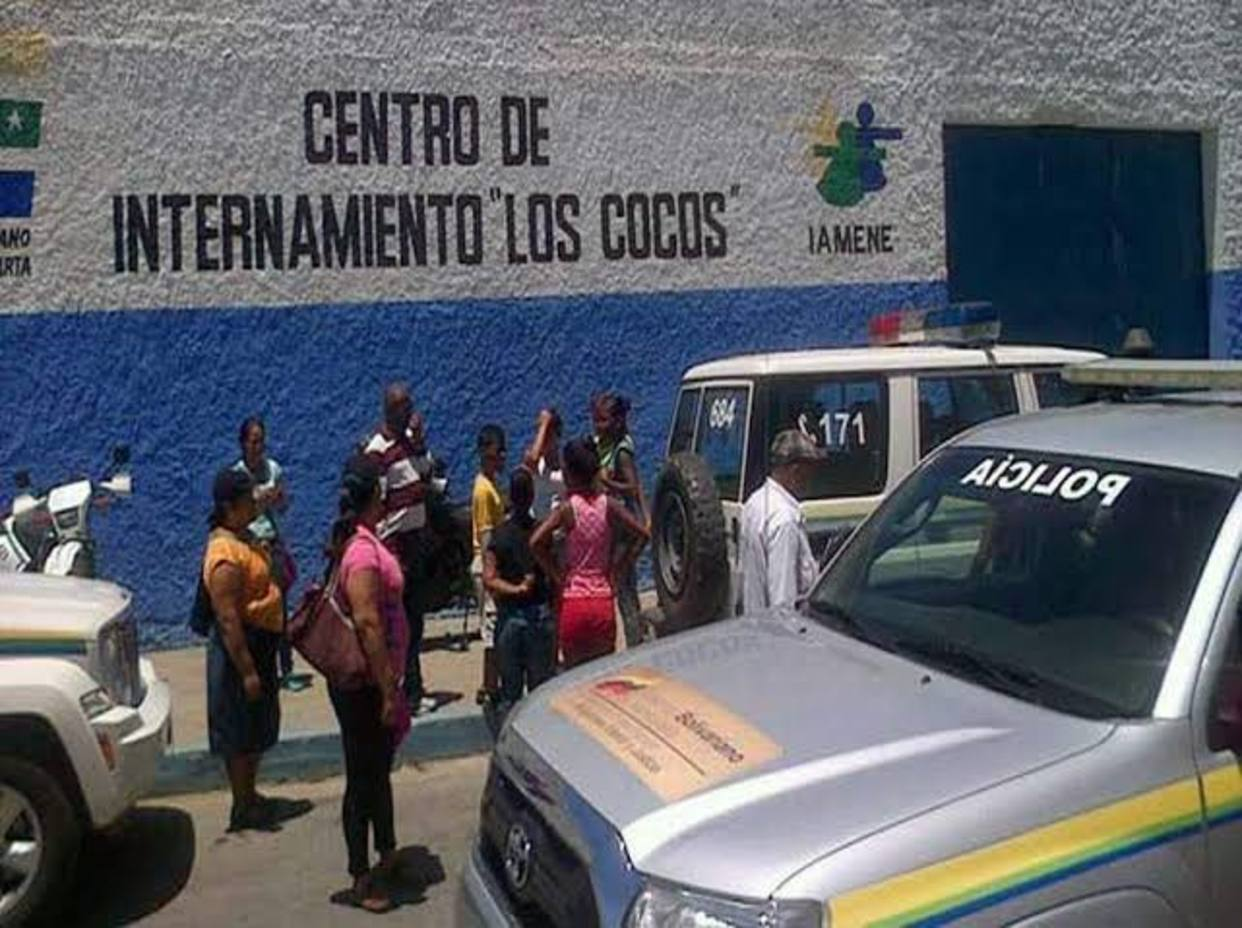
\includegraphics[width=300px]{115.jpg}%
\newline%
%
Este domingo, se fugaron al menos 30 personas del retén de adultos Los Cocos en Porlamar, estado Nueva Esparta, información que fue confirmada horas después de que se reportaran unas detonaciones en el lugar.%
\newline%
%
"Se calculan que se lograron escapar más de 30 reclusos del retén de adultos en Los Cocos en Porlamar. Aún están contabilizando la cantidad exacta de fugados. Hay dos muertos entre los reclusos durante intento de fuga", informó el programa de radio local "Bajo La Lupa".%
\newline%
%
Desde tempranas horas de este domingo, corrían rumores en las redes sociales con respecto a este suceso, pero las autoridades pertinentes no se pronunciaron al respecto.%
\newline%
%
El plan de recaptura de los presos que se escaparon se aplicará en las próximas horas.%
\newline%
%
\end{document}